% Workflow diagram (Figure 2). Build: cd figures && pdflatex diagram.tex
% Thumbnails in diagram_img/ are crops of occlusion_ex.jpg.
\documentclass[tikz,border=2pt]{standalone}
\usetikzlibrary{arrows.meta,positioning,calc}
\definecolor{cmodal}{RGB}{52,101,164}
\definecolor{cbody}{RGB}{56,142,60}
\definecolor{cocc}{RGB}{214,120,30}
\definecolor{cbg}{RGB}{120,90,160}
\definecolor{cout}{RGB}{190,50,50}
\begin{document}
\sffamily
\begin{tikzpicture}[
  >={Stealth[length=2mm]},
  arr/.style={->, thick, draw=black!65},
  thumb/.style={inner sep=0pt, draw=#1, line width=1.2pt},
  ttl/.style={font=\footnotesize\bfseries, text=#1, align=center, anchor=south},
  sub/.style={font=\scriptsize, text=black!75, align=center, anchor=north, text width=21mm},
  lab/.style={font=\scriptsize\itshape, text=black!70, fill=white, inner sep=1pt},
  sec/.style={font=\scriptsize, text=black!55}]
  \def\W{1.85cm}
  % ---- main row
  \foreach \n/\img/\x/\c in {in/input/0/black!60, mod/modal/2.2/cmodal, bod/meshes/4.4/cbody,
                             amo/amodal/6.6/cbody, occ/occlusion/8.8/cocc, out/composite/11/cout}{
    \node[thumb=\c] (\n) at (\x,0) {\includegraphics[width=\W]{diagram_img/\img.jpg}};
  }
  \node[ttl=black!70] at (in.north)  {Input image\\[-1pt]\phantom{g}};
  \node[ttl=cmodal]   at (mod.north) {Modal masks\\[-1pt]{\mdseries\scriptsize per person}};
  \node[ttl=cbody]    at (bod.north) {3D bodies\\[-1pt]{\mdseries\scriptsize per person}};
  \node[ttl=cbody]    at (amo.north) {Amodal masks\\[-1pt]{\mdseries\scriptsize $A_j$ + depth $D_j$}};
  \node[ttl=cocc]     at (occ.north) {Occlusion masks\\[-1pt]{\mdseries\scriptsize $O_j = A_j \land \lnot V_i$}};
  \node[ttl=cout]     at (out.north) {De-occluded\\[-1pt]composite};
  \node[sub] at (mod.south) {YOLO11 + SAM~2\\{\color{black!55}Sec.~3}};
  \node[sub] at (bod.south) {SAM 3D Body\\{\color{black!55}Sec.~4}};
  \node[sub] at (amo.south) {projection +\\z-buffer\quad{\color{black!55}Sec.~4}};
  \node[sub] at (occ.south) {matching, opening,\\person/object label\\{\color{black!55}Sec.~5}};
  \node[sub] at (out.south) {meshes over\\background\\{\color{black!55}Sec.~7}};
  % ---- main arrows
  \draw[arr] (in) -- (mod);
  \draw[arr] (mod) -- (bod);
  \draw[arr] (bod) -- (amo);
  \draw[arr] (amo) -- (occ);
  \draw[arr] (occ) -- (out);
  % modal masks also feed the occlusion step (V)
  \draw[arr, draw=cmodal!80] ($(mod.north)+(0.45,0.75)$) -- ++(0,0.35) -| node[pos=0.25, lab, text=cmodal]{visible masks $V_i$} ($(occ.north)+(-0.45,0.75)$);
  % ---- second row: cross-model detection and background
  \node[draw=cmodal, fill=cmodal!8, rounded corners=3pt, align=center, font=\scriptsize,
        text width=24mm, inner sep=2pt] (mhr) at (0.75,-2.55)
        {\textbf{Multi-HMR}\\finds people missed\\by YOLO11 (Sec.~5)};
  \draw[arr] ($(in.south)+(0.75,0)$) -- ($(mhr.north)+(0,0)$);
  \draw[arr, draw=cmodal!80] (mhr.east) -| ($(mod.south)+(-0.15,-0.95)$);
  \node[thumb=cbg] (bg) at (8.8,-2.85) {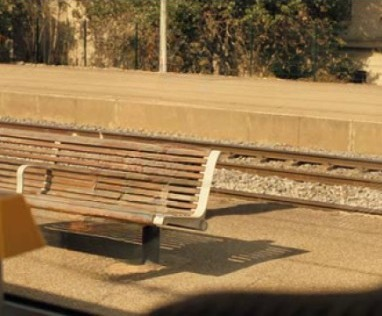
\includegraphics[width=\W]{diagram_img/background.jpg}};
  \node[ttl=cbg, anchor=east] at ($(bg.west)+(-0.1,0.2)$) {Background};
  \node[font=\scriptsize, text=black!75, anchor=east, align=right] at ($(bg.west)+(-0.1,-0.3)$) {LaMa inpainting\quad{\color{black!55}Sec.~6}};
  \draw[arr, draw=cbg!80] ($(mod.south)+(0.6,-0.95)$) |- (bg.west);
  \draw[arr, draw=cbg!80] (bg.east) -| ($(out.south)+(0,-1.05)$);
\end{tikzpicture}
\end{document}
